%
% Chapter 8 — Current State and Future Work
%
\chapter{Current State and Future Work} \label{cap:currentstate}

This report describes the beta version of the platform. While the architecture,
data model, and core application components have been defined and largely
implemented, some requirements presented in Chapter 3 remain under development
and are planned for completion in the final version. The following sections
summarise the work accomplished so far and the remaining tasks.

\section{Accomplished Work} \label{sec:conc_accomplished}

\begin{itemize}
      \item \textbf{Architecture and data model}: the system architecture was defined,
            the technology stack selected, and the database schema designed and implemented,
            including support for a block-based content model, media credits, category
            hierarchy, and session management.

      \item \textbf{Authentication}: a JWT-based authentication mechanism was implemented,
            with short-lived access tokens and long-lived refresh tokens stored as
            \texttt{HttpOnly} cookies. Token refresh is handled transparently on the
            frontend.

      \item \textbf{Backend API}: the REST API covers user management,
            invitation-based onboarding, category and tag management, media upload and
            management, and content creation. The editorial workflow is currently under
            active development.

      \item \textbf{Content editor}: the backoffice content editor is functional,
            supporting block-based authoring with text and image blocks, inline formatting,
            media gallery integration, and metadata configuration (category, tags, authors,
            slug). Support for video content is implemented; podcast and episode creation
            are in an advanced stage of development.

      \item \textbf{Backoffice}: the backoffice interface is largely implemented, covering
            content listing, user management with filters, category and tag management,
            invitation management, and user profiles.

      \item \textbf{Public website}: the article page is implemented and functional.
            The homepage is under active development, currently rendered with mocked data.
            The shared components used across public pages are already in place.

      \item \textbf{Testing and CI}: backend and frontend test suites are in development and
            integrated into a continuous integration pipeline via GitHub Actions.
\end{itemize}

\section{Remaining Work} \label{sec:conc_future}

Figure~\ref{fig:gantt} presents the project timeline, showing completed,
in-progress, and planned tasks up to the final delivery on 11 July 2026.

\begin{figure}[H]
      \begin{center}
            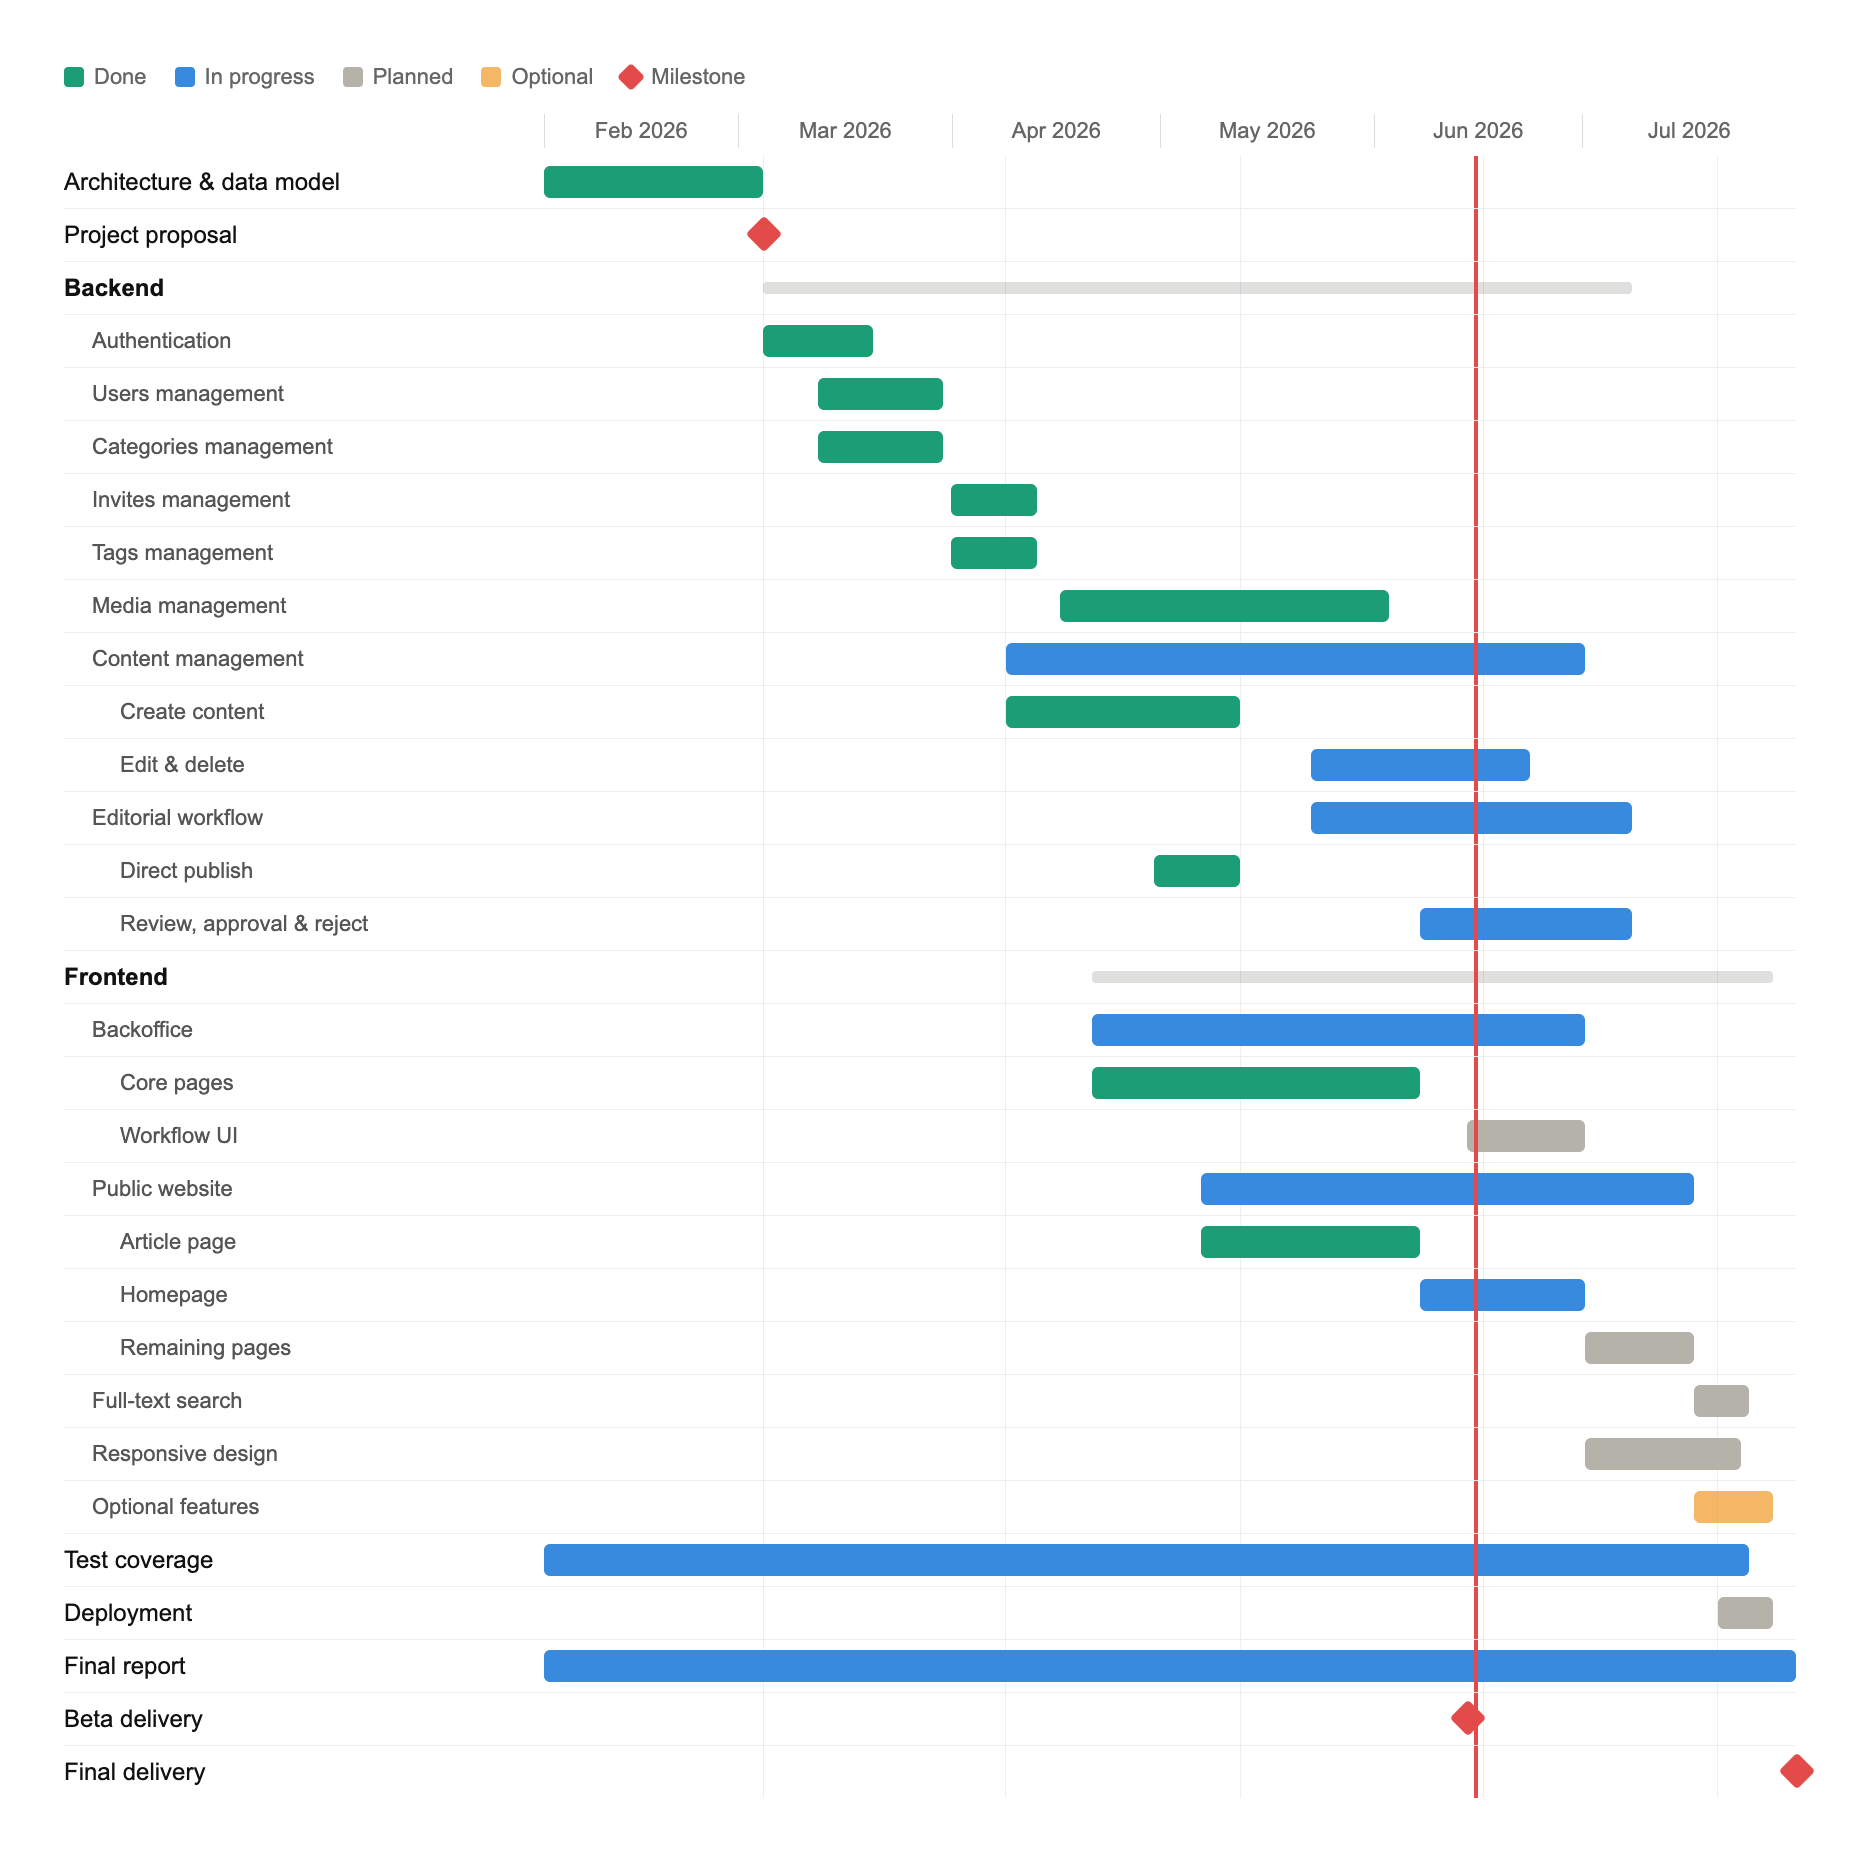
\includegraphics[width=\textwidth]{./figures/gantt.png}
      \end{center}
      \caption{Project Gantt chart.}
      \label{fig:gantt}
\end{figure}

The following items are planned for the final version:

\begin{itemize}
      \item \textbf{Editorial workflow}: complete the submission, approval, and
            rejection workflow in both the backend and the backoffice interface,
            including a dedicated pending content view for Editors.

      \item \textbf{Public website}: complete the homepage with real data and
            connect the remaining pages --- category listings, tag listings, podcast
            page, and author profile page --- to the API. The shared components are
            already implemented; the remaining work consists primarily of page
            assembly and API integration.

      \item \textbf{Full-text search}: implement keyword search across published
            content, accessible from the public website.

      \item \textbf{Responsive design}: complete the responsive layout across all
            viewports only for the public website.

      \item \textbf{Test coverage}: expand automated test coverage across backend
            and frontend layers.

      \item \textbf{Deployment}: deploy the application to the IPL server
            infrastructure, with a dedicated section documenting the deployment
            process and maintenance procedures.

      \item \textbf{Optional features}: reader comments, advanced search
            filters, and a scheduled publication date picker (the data model
            already supports scheduled publication via future
            \texttt{published\_at} timestamps), subject to available time.
\end{itemize}

\section{Limitations}

As this report describes the beta version of the platform, some aspects of the
system remain incomplete or have not yet been validated under production
conditions. While the core architecture, data model, authentication mechanism,
and content management capabilities are operational, several components are
still undergoing development and refinement.

The editorial workflow has been defined at the architectural level, but
some workflow transitions and supporting backoffice interfaces are still being
completed. Similarly, although the public website structure has been
implemented, parts of the homepage and several listing pages currently rely on
mocked data pending full integration with the backend services.

Testing activities are also at an early stage. Unit, integration, and
end-to-end test suites have been established and integrated into the continuous
integration pipeline, but overall test coverage remains limited. Consequently,
the platform has not yet been validated against the full range of functional
and non-functional requirements.

Finally, the system has not yet been deployed to the target IPL
infrastructure. As a result, aspects such as operational monitoring, backup
procedures, deployment automation, and real-world performance characteristics
have not yet been evaluated.
